%\chapter{METODOLOGIA}
%\label{metodologia}
%--------------------------------------------------------------
\chapter{\textbf{MODELAGEM NUMÉRICA}}
\label{sec_modelagem}

%--------------------------------------------------------------
\section{\textbf{Introdução}}
Neste trabalho foram utilizados dois tipos de modelagem numéricas para simular o comportamento do sistema multifásico.
Na fase dos fluidos, foi utilizado o \hyperref[mef]{\textit{Método de Elementos Finitos} (MEF)} para solucionar as equações de governo, pois ele proporciona uma forma eficiente de solucionar as equações com rápida convergência.
Enquanto para a fase sólida das partículas, e o termo temporal das equações dos fluidos, foi utilizado o \hyperref[mdf]{\textit{Método de Diferenças Finitas} (MDF)}, o qual foi escolhido por sua simplicidade de implementação tomando-se cuidado com suas restrições de convergência.


%--------------------------------------------------------------
\section{\textbf{Método de Elementos Finitos}}
\label{mef}
%--------------------------------------------------------------
\subsection{\textbf{Formulação Forte}}
\label{form_forte}
A formulação forte são as equações de governo do problema na sua forma diferencial, com as condições de contorno definidas.
As equações do fluido definidas em \refeq{fluid_eq1}, \refeq{fluid_eq2} e \refeq{fluid_eq3} são tomadas no domínio $\Omega \subset \mathbb{R}^2$ com condições de contorno definidas em:
\begin{align}
    \omega &= \omega_{\Gamma} \text{ em } \Gamma_1 \\
    \psi &= \psi_{\Gamma} \text{ em } \Gamma_2 \\
    \vec{v}_f &= \vec{v}_{f\Gamma} \text{ em } \Gamma_3 
\end{align}

%--------------------------------------------------------------
\subsection{\textbf{Formulação Fraca}}
A formulação fraca é o resultado da ponderação da equação da forma forte integrada sobre o domínio.
Para o encontrar as formas fracas das equações de governo tomadas neste trabalho, inicialmente são estabelecidos resíduos $\vec{R_i}$ nas equações de forma forte:
\begin{equation}
    \dfrac{\partial \vec{\omega}}{\partial t} +
    \vec{v}_f.\vec{\nabla}.\vec{\omega} -
    \dfrac{\mu_f}{\rho_f} \nabla^2 \vec{\omega} =
    \vec{R_1}
\end{equation}
\begin{equation}
    \nabla^2\psi +
    \omega_z =
    \vec{R_2}
\end{equation}
\begin{equation}
    \vec{v}_f - \left(\dfrac{\partial \psi}{\partial y},
    -\dfrac{\partial \psi}{\partial x} \right) =
    \vec{R_3}
\end{equation}

Em seguida, busca-se impor o valor médio de cada resíduo como nulo, de forma que:
\begin{align}
    \int_{\Omega} \vec{R_1} . \vec{\delta} d\Omega = 0 \\
    \int_{\Omega} \vec{R_2} . \vec{\phi} d\Omega = 0\\
    \int_{\Omega} \vec{R_3} . \vec{\xi} d\Omega = 0
\end{align}
onde $\vec{\delta}$, $\vec{\phi}$ e $\vec{\xi}$ são as funções de peso de cada equação, respectivamente.
As funções peso são funções arbitrárias utilizadas para obter as componentes de contribuição de cada nó.

Substituindo-se os resíduos nas integrais, tem-se:
\begin{equation}
    \int_{\Omega} \left(
    \dfrac{\partial \vec{\omega}}{\partial t} +
    \vec{v}_f.\vec{\nabla}.\vec{\omega} -
    \dfrac{\mu_f}{\rho_f} \nabla^2 \vec{\omega}
    \right).\vec{\delta} d\Omega = 0
\end{equation}
\begin{equation}
    \int_{\Omega} \left(
    \nabla^2\psi +
    \omega_z
    \right).\vec{\phi} d\Omega = 0
\end{equation}
\begin{equation}
    \int_{\Omega} \left(
    \vec{v}_f - \left(\dfrac{\partial \psi}{\partial y},
    -\dfrac{\partial \psi}{\partial x} \right)
    \right).\vec{\xi} d\Omega = 0
\end{equation}

Reorganiza-se as integrais:
\begin{equation}
    \int_{\Omega}
    \dfrac{\partial \vec{\omega}}{\partial t}
    .\vec{\delta} d\Omega +
    \int_{\Omega}
    \vec{v}_f.\vec{\nabla}.\vec{\omega}
    .\vec{\delta} d\Omega -
    \int_{\Omega}
    \dfrac{\mu_f}{\rho_f} \nabla^2 \vec{\omega}
    .\vec{\delta} d\Omega = 0
\end{equation}
\begin{equation}
    \int_{\Omega}
    \nabla^2\psi
    .\vec{\phi} d\Omega +
    \int_{\Omega}
    \omega_z
    .\vec{\phi} d\Omega = 0
\end{equation}
\begin{equation}
    \int_{\Omega}
    \vec{v}_f
    .\vec{\xi} d\Omega -
    \int_{\Omega}
    \left(\dfrac{\partial \psi}{\partial y},
    -\dfrac{\partial \psi}{\partial x} \right)
    .\vec{\xi} d\Omega = 0
\end{equation}

Aplica-se agora o Teorema de Green nos termos difusivos das equações:
\begin{equation}
    -\int_{\Omega}
    \dfrac{\mu_f}{\rho_f} \nabla^2 \vec{\omega}
    .\vec{\delta} d\Omega = 
    \int_{\Omega}
    \dfrac{\mu_f}{\rho_f}
    \vec{\nabla}.\vec{\omega}.\vec{\nabla}
    .\vec{\delta} d\Omega -
    \int_{\Gamma}
    \dfrac{\mu_f}{\rho_f}
    \vec{\delta}.\vec{\nabla}.\vec{\omega}
    .\vec{n} d\Gamma
\end{equation}
\begin{equation}
    \int_{\Omega}
    \nabla^2\psi
    .\vec{\phi} d\Omega = -
    \int_{\Omega}
    \vec{\nabla}.\psi.\vec{\nabla}
    .\vec{\phi} d\Omega +
    \int_{\Gamma}
    \vec{\phi}.\vec{\nabla}.\psi
    .\vec{n} d\Gamma
\end{equation}
onde $\vec{n}$ é um vetor normal unitário, orientado para o exterior do contorno $\Gamma$.
Como as condições de contorno definidas para o problema em \ref{form_forte} apontam apenas condições de Dirichlet, isto é, valores fixos no contorno, pode-se assumir como hipótese que $\delta=0$ e $\phi=0$ em todo o contorno $\Gamma$.
Assim, a integral em $\Gamma$ é nula e os termos difusivos são anulados:
\begin{equation}
    -\int_{\Omega}
    \dfrac{\mu_f}{\rho_f} \nabla^2 \vec{\omega}
    .\vec{\delta} d\Omega = 
    \int_{\Omega}
    \dfrac{\mu_f}{\rho_f}
    \vec{\nabla}.\vec{\omega}.\vec{\nabla}
    .\vec{\delta} d\Omega
\end{equation}
\begin{equation}
    \int_{\Omega}
    \nabla^2\psi
    .\vec{\phi} d\Omega = -
    \int_{\Omega}
    \vec{\nabla}.\psi.\vec{\nabla}
    .\vec{\phi} d\Omega
\end{equation}

As equações ficam então como:
\begin{equation}
    \int_{\Omega}
    \dfrac{\partial \vec{\omega}}{\partial t}
    .\vec{\delta} d\Omega +
    \int_{\Omega}
    \vec{v}_f.\vec{\nabla}.\vec{\omega}
    .\vec{\delta} d\Omega +
    \int_{\Omega}
    \dfrac{\mu_f}{\rho_f}
    \vec{\nabla}.\vec{\omega}.\vec{\nabla}
    .\vec{\delta} d\Omega= 0
\end{equation}
\begin{equation}
    -\int_{\Omega}
    \vec{\nabla}.\psi.\vec{\nabla}
    .\vec{\phi} d\Omega +
    \int_{\Omega}
    \omega_z
    .\vec{\phi} d\Omega = 0
\end{equation}
\begin{equation}
    \int_{\Omega}
    \vec{v}_f
    .\vec{\xi} d\Omega -
    \int_{\Omega}
    \left(\dfrac{\partial \psi}{\partial y},
    -\dfrac{\partial \psi}{\partial x} \right)
    .\vec{\xi} d\Omega = 0
\end{equation}

Se assumir-se que:
\begin{equation}
    m_1 \left(\dfrac{\partial \vec{\omega}}{\partial t}, \delta\right) =
    \int_{\Omega}
    \dfrac{\partial \vec{\omega}}{\partial t}
    .\vec{\delta} d\Omega
\end{equation}
\begin{equation}
    g_1 (\vec{v}_f, \vec{\delta}) =
    \int_{\Omega}
    \vec{v}_f.\vec{\nabla}.\vec{\omega}
    .\vec{\delta} d\Omega
\end{equation}
\begin{equation}
    k_1 (\vec{\omega}, \vec{\delta}) =
    \int_{\Omega}
    \vec{\nabla}.\vec{\omega}.\vec{\nabla}
    .\vec{\delta} d\Omega
\end{equation}
\begin{equation}
    k_2 (\psi, \vec{\phi}) =
    \int_{\Omega}
    \vec{\nabla}.\psi.\vec{\nabla}
    .\vec{\phi} d\Omega
\end{equation}
\begin{equation}
    m_2 (\omega_z, \vec{\phi}) =
    \int_{\Omega}
    \omega_z
    .\vec{\phi} d\Omega
\end{equation}
\begin{equation}
    m_3 (\vec{v}_f, \vec{\xi}) =
    \int_{\Omega}
    \vec{v}_f
    .\vec{\xi} d\Omega
\end{equation}
\begin{equation}
    g_3 (\psi, \vec{\xi}) =
    \int_{\Omega}
    \left(\dfrac{\partial \psi}{\partial y},
    -\dfrac{\partial \psi}{\partial x} \right)
    .\vec{\xi} d\Omega
\end{equation}
então as equações na forma fraca são:
\begin{align}
    m_1 \left(\dfrac{\partial \vec{\omega}}{\partial t}, \delta\right) +
    g_1 (\vec{v}_f, \vec{\delta}) + 
    \dfrac{\mu_f}{\rho_f} k_1 (\vec{\omega}, \vec{\delta}) &=0\\
    -k_2 (\psi, \vec{\phi}) +
    m_2 (\omega_z, \vec{\phi}) &= 0 \\
    m_3 (\vec{v}_f, \vec{\xi}) - 
    g_3 (\psi, \vec{\xi}) &=0
\end{align}

Para os seguintes conjuntos de funções bases:
\begin{align}
    \mathbb{W}&=\left\{\omega \in \Omega \rightarrow \mathbb{R}^2: 
    \int_{\Omega} \omega^2 d\Omega < \infty; \omega \in \omega_{\Gamma}\right\} \\
    \mathbb{P}&=\left\{\psi \in \Omega \rightarrow \mathbb{R}^2: 
    \int_{\Omega} \psi^2 d\Omega < \infty; \psi \in \psi_{\Gamma}\right\} \\
    \mathbb{V}&=\left\{v_f \in \Omega \rightarrow \mathbb{R}^2: 
    \int_{\Omega} v_f^2 d\Omega < \infty; v_f \in v_{f\Gamma}\right\}
\end{align}


%--------------------------------------------------------------
\subsection{\textbf{Discretização Espacial}}
A escolha das funções peso pode ser realizada de várias formas, por simplicidade este trabalho utiliza a \textbf{Formulação de Galerkin}.
Neste método, as funções peso são utilizadas com o mesmo valor da função interpoladora de cada variável. 
Substituindo-se nas equações:
\begin{align}
    \int_{\Omega}
    \dfrac{\partial \omega}{\partial t}
    \delta d\Omega &+
    \int_{\Omega}
    v_{fx}\dfrac{\partial \omega}{\partial x}
    \delta d\Omega +
    \int_{\Omega}
    v_{fy}\dfrac{\partial \omega}{\partial y}
    \delta d\Omega \nonumber\\&+
    \int_{\Omega}
    \dfrac{\mu_f}{\rho_f}
    \left(
    \dfrac{\partial \omega}{\partial x}
    \dfrac{\partial \delta}{\partial x} +
    \dfrac{\partial \omega}{\partial y}
    \dfrac{\partial \delta}{\partial y}
    \right) d\Omega= 0
\end{align}
\begin{equation}
    -\int_{\Omega}
    \left(
    \dfrac{\partial \psi}{\partial x}
    \dfrac{\partial \phi}{\partial x} +
    \dfrac{\partial \psi}{\partial y}
    \dfrac{\partial \phi}{\partial y}
    \right) d\Omega +
    \int_{\Omega}
    \omega_z
    \phi d\Omega = 0
\end{equation}
\begin{equation}
    \int_{\Omega}
    v_{fx}
    \xi d\Omega -
    \int_{\Omega}
    \dfrac{\partial \psi}{\partial y}
    \xi d\Omega = 0
\end{equation}
\begin{equation}
    \int_{\Omega}
    v_{fy}
    \xi d\Omega +
    \int_{\Omega}
    \dfrac{\partial \psi}{\partial x}
    \xi d\Omega = 0
\end{equation}

As discretizações são aplicadas sobre um domínio com $n_e$ elementos e $n_p$ nós.
Este domínio é determinado por uma malha computacional criada.
As variáveis ficam então:

\begin{align}
    \omega(\vec{x}, t) &= \sum_{i=1}^{n_p} \omega_i(t) N_i(\vec{x}) \\
    \psi(\vec{x}, t) &= \sum_{i=1}^{n_p} \psi_i(t) N_i(\vec{x}) \\
    v_{fx}(\vec{x}, t) &= \sum_{i=1}^{n_p} v_{fxi}(t) N_i(\vec{x}) \\
    v_{fy}(\vec{x}, t) &= \sum_{i=1}^{n_p} v_{fyi}(t) N_i(\vec{x}) 
\end{align}
onde os valores das funções em cada ponto $\omega_i = [\omega_1, \ldots, \omega_{n_p}]$, $\psi_i = [\psi_1, \ldots, \psi_{n_p}]$, $v_{fxi} = [v_{fx1}, \ldots, v_{fxn_p}]$ e $v_{fyi} = [v_{fy1}, \ldots, v_{fyn_p}]$ são as incógnitas desejadas.
Como estas funções são independentes do tempo, elas são retiradas dos termos de integração sobre o domínio $\Omega$.
Enquanto isso, as funções de aproximação $N_{i} = [N_{1}, \ldots, N_{n_p}]$, também chamadas de funções base, são escolhidas arbitrariamente.

Na formulação de Galerkin, as funções de base são iguais as suas respectivas funções peso:
\begin{align}
    \delta(\vec{x}, t) &= \sum_{j=1}^{n_p} \delta_i(t) N_j(\vec{x}) \\
    \phi(\vec{x}, t) &= \sum_{j=1}^{n_p} \phi_i(t) N_j(\vec{x}) \\
    \xi(\vec{x}, t) &= \sum_{j=1}^{n_p} \xi_i(t) N_j(\vec{x})
\end{align}

Então as equações do sistema em suas formas variacionais discretizadas no espaço ficam como:
\begin{align}
    &\int_{\Omega}
    \sum_{i=1}^{n_p} \dfrac{\partial \omega_i}{\partial t} N_i
    \sum_{j=1}^{n_p} \delta_j N_j
    d\Omega \nonumber\\&+
    \int_{\Omega}
    v_{fx}
    \sum_{i=1}^{n_p} \dfrac{\partial \omega_i N_i}{\partial x}
    \sum_{j=1}^{n_p} \delta_j N_j
    d\Omega +
    \int_{\Omega}
    v_{fy}
    \sum_{i=1}^{n_p} \dfrac{\partial \omega_i N_i}{\partial y}
    \sum_{j=1}^{n_p} \delta_j N_j
    d\Omega \nonumber\\&+
    \int_{\Omega}
    \dfrac{\mu_f}{\rho_f}
    \left(
    \sum_{i=1}^{n_p} \dfrac{\partial \omega_i N_i}{\partial x}
    \sum_{j=1}^{n_p} \dfrac{\partial \delta_j N_j}{\partial x} +
    \sum_{i=1}^{n_p} \dfrac{\partial \omega_i N_i}{\partial y}
    \sum_{j=1}^{n_p} \dfrac{\partial \delta_j N_j}{\partial y}
    \right) d\Omega= 0
    \label{temp1}
\end{align}
\begin{align}
    -\int_{\Omega}
    \left(
    \sum_{i=1}^{n_p} \dfrac{\partial \psi_i N_i}{\partial x}
    \sum_{j=1}^{n_p} \dfrac{\partial \phi_j N_j}{\partial x} +
    \sum_{i=1}^{n_p} \dfrac{\partial \psi_i N_i}{\partial y}
    \sum_{j=1}^{n_p} \dfrac{\partial \phi_j N_j}{\partial y}
    \right) d\Omega \nonumber\\+
    \int_{\Omega}
    \sum_{i=1}^{n_p} \omega_{zi} N_i
    \sum_{j=1}^{n_p} \phi_j N_j
    d\Omega = 0
\end{align}
\begin{equation}
    \int_{\Omega}
    \sum_{i=1}^{n_p} v_{fxi} N_i
    \sum_{j=1}^{n_p} \xi_j N_j
    d\Omega -
    \int_{\Omega}
    \sum_{i=1}^{n_p} \dfrac{\partial \psi_i N_i}{\partial y}
    \sum_{j=1}^{n_p} \xi_j N_j
    d\Omega = 0
\end{equation}
\begin{equation}
    \int_{\Omega}
    \sum_{i=1}^{n_p} v_{fyi} N_i
    \sum_{j=1}^{n_p} \xi_j N_j
    d\Omega +
    \int_{\Omega}
    \sum_{i=1}^{n_p} \dfrac{\partial \psi_i N_i}{\partial x}
    \sum_{j=1}^{n_p} \xi_j N_j
    d\Omega = 0
\end{equation}

Pode-se remover as componentes da velocidade do fluido $v_{fx}$ e $v_{fy}$ da equação \refeq{temp1}, pois serão utilizados os componentes da velocidade no último passo de tempo para estes valores, tornando-se a equação linear.

Retira-se então os somatórios das funções interpoladoras das integrais, e como $\sum_{j=1}^{n_p} \delta_j \neq 0$, $\sum_{j=1}^{n_p} \phi_j \neq 0$ e $\sum_{j=1}^{n_p} \xi_j \neq 0$ as equações de governo serão:
\begin{align}
    &\sum_{j=1}^{n_p}
    \sum_{i=1}^{n_p} \dfrac{\partial \omega_i}{\partial t}
    \int_{\Omega}
    N_i N_j
    d\Omega \nonumber\\&+
    \sum_{j=1}^{n_p}
    \sum_{i=1}^{n_p}
    \omega_i
    \left(
        v_{fx}
        \int_{\Omega}
        \dfrac{\partial N_i}{\partial x}
        N_j
        d\Omega +
        v_{fy}
        \int_{\Omega}
        \dfrac{\partial N_i}{\partial y}
        N_j
        d\Omega \right.\nonumber\\ +& \left.
        \dfrac{\mu_f}{\rho_f}
        \int_{\Omega}
        \dfrac{\partial N_i}{\partial x}
        \dfrac{\partial N_j}{\partial x} +
        \dfrac{\partial N_i}{\partial y}
        \dfrac{\partial N_j}{\partial y}
        d\Omega
    \right) = 0
\end{align}
\begin{align}
    \sum_{j=1}^{n_p}
    \sum_{i=1}^{n_p}
    \psi_i
    \left(
        -\int_{\Omega} \left(
        \dfrac{\partial N_i}{\partial x}
        \dfrac{\partial N_j}{\partial x} +
        \dfrac{\partial N_i}{\partial y}
        \dfrac{\partial N_j}{\partial y}
        \right) d\Omega +
        \omega_i
        \int_{\Omega}
        N_i
        N_j
        d\Omega +
    \right) = 0
\end{align}
\begin{equation}
    \sum_{j=1}^{n_p}
    \sum_{i=1}^{n_p}
    v_{fxi}
    \left(
        \int_{\Omega}
        N_i
        N_j
        d\Omega -
        \psi_i
        \int_{\Omega}
        \dfrac{\partial N_i}{\partial y}
        N_j
        d\Omega +
    \right) = 0
\end{equation}
\begin{equation}
    \sum_{j=1}^{n_p}
    \sum_{i=1}^{n_p}
    v_{fyi}
    \left(
        \int_{\Omega}
        N_i
        N_j
        d\Omega +
        \psi_i
        \int_{\Omega}
        \dfrac{\partial N_i}{\partial x}
        N_j
        d\Omega +
    \right) = 0
\end{equation}

%--------------------------------------------------------------
\subsection{\textbf{Malha Computacional}}
A malha utilizada pode ser estruturada, com nós equidistantes entre si, ou não estruturada, nós escolhidos a critério do criador da malha.
É comum utilizar malhas não estruturadas com zonas de maior interesse com elementos menores, para se obter informações mais precisas nestes locais.
Em certos casos de equações com acoplamentos fortemente ligados, se torna necessário utilizar elementos com mais informações atreladas, como elementos quadráticos ou cúbicos.
Este é o caso da solução da equação de Navier-Stoakes.
Porém, para evitar esta restrição, este trabalho utilizou a formulação de corrente-vorticidade, que desvia deste problema.
Podendo então utilizar elementos lineares e simplificando sua implementação.

Os tipos de elementos mais comuns aplicados a aos diferentes tipos de simulações são \cite{gustavo}:
\begin{itemize}
    \item Dimensão do problema
    \begin{itemize}
        \item[-] Caso unidimensional: Retas
        \item[-] Caso bidimensional: Triângulos ou Retângulos
        \item[-] Caso tridimensional: Tetraedros ou Prismas
    \end{itemize}
    \item Ordem dos polinômios interpoladores
    \begin{itemize}
        \item[-] Primeiro grau: Lineares 
        \item[-] Segundo grau: Quadráticos
        \item[-] Terceiro grau: Cúbicos
    \end{itemize}
\end{itemize}

Para este trabalho foi escolhido o elemento do tipo triangular com interpolação linear, pois não há restições no problema escolhido, e este é o caso mais aplicado na literatura.
A \ref{element} mostra como são os elementos utilizados:
\begin{figure}[H]
    \centering
    \stackunder{
        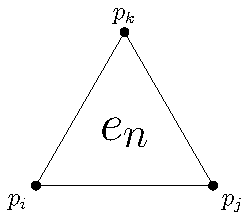
\includegraphics[width=0.5\linewidth]{figures/element.pdf}
    } {\raggedleft \scriptsize Fonte: Autor.}
    \caption{Elemento triangular linear.}
    \label{element}
\end{figure}

Pode-se notar na \ref{element} que o elemento de índice $e_n$ é delimitado pelos nós $p_i$, $p_j$ e $p_k$.
A função de interpolação aplicada entre os nós é uma função linear entre suas posições.

Então pode-se escrever as equações do problema em sua forma matricial como:
\begin{equation}
    \mathbf{M}
    \dfrac{\partial \omega}{\partial t} +
    v_{fx}
    \mathbf{G_x}
    \omega +
    v_{fy}
    \mathbf{G_y}
    \omega +
    \dfrac{\mu_f}{\rho_f}
    \left(
    \mathbf{K_{xx}} +
    \mathbf{K_{yy}}
    \right)
    \omega = 0
    \label{last_dt}
\end{equation}
\begin{equation}
    -\left(
    \mathbf{K_{xx}} +
    \mathbf{K_{yy}}
    \right)
    \psi +
    \mathbf{M}
    \omega = 0
\end{equation}
\begin{equation}
    \mathbf{M}
    v_{fx}
    \omega -
    \mathbf{G_y}
    \psi = 0
\end{equation}
\begin{equation}
    \mathbf{M}
    v_{fy}
    \omega +
    \mathbf{G_x}
    \psi = 0
\end{equation}
onde $\mathbf{M}$, $\mathbf{G_{x}}$, $\mathbf{G_{y}}$, $\mathbf{K_{xx}}$ e $\mathbf{K_{yy}}$ são as matrizes elementares de dimensão $n_p \times n_p$.

Estas matrizes são montadas a partir da contribuição local de cada nó em um elemento e unidas na matriz geral, onde cada posição da matriz é o valor correspondente ao nó de mesmo índice.
As matrizes locais $\mathbf{m^e}$, $\mathbf{g_{x}^e}$, $\mathbf{g_{y}^e}$, $\mathbf{k_{xx}^e}$ e $\mathbf{k_{yy}^e}$, para cada elemento $e$ são definidas como:
\begin{align}
    \mathbf{m^e} &=
    \int_{\Omega^e}
    N_i^e N_j^e
    d\Omega^e \\
    \mathbf{g_x^e} &=
    \int_{\Omega^e}
    \dfrac{\partial N_i^e}{\partial x}
    N_j^e
    d\Omega^e \\
    \mathbf{g_y^e} &=
    \int_{\Omega^e}
    \dfrac{\partial N_i^e}{\partial y}
    N_j^e
    d\Omega^e \\
    \mathbf{k_{xx}^e} &=
    \int_{\Omega^e}
    \dfrac{\partial N_i^e}{\partial x}
    \dfrac{\partial N_j^e}{\partial x}
    d\Omega^e \\
    \mathbf{k_{yy}^e} &=
    \int_{\Omega^e}
    \dfrac{\partial N_i^e}{\partial y}
    \dfrac{\partial N_j^e}{\partial y}
    d\Omega^e
\end{align}

Esctritas em suas formas matriciais\cite{lewis}:
\begin{align}
    \mathbf{m^e} &=
    \dfrac{A^e}{12}
    \begin{bmatrix} 
        2 & 1 & 1 \\
        1 & 2 & 1 \\
        1 & 1 & 2
    \end{bmatrix} \\
    \mathbf{g_x^e} &=
    \dfrac{1}{6}
    \begin{bmatrix} 
        b_i & b_j & b_k \\
        b_i & b_j & b_k \\
        b_i & b_j & b_k
    \end{bmatrix} \\
    \mathbf{g_y^e} &=
    \dfrac{1}{6}
    \begin{bmatrix} 
        c_i & c_j & c_k \\
        c_i & c_j & c_k \\
        c_i & c_j & c_k
    \end{bmatrix} \\
    \mathbf{k_{xx}^e} &=
    \dfrac{t_h}{4A}
    \begin{bmatrix} 
        b_i b_i & b_j b_i & b_k b_i \\
        b_i b_j & b_j b_j & b_k b_j \\
        b_i b_k & b_j b_k & b_k b_k
    \end{bmatrix} \\
    \mathbf{k_{yy}^e} &=
    \dfrac{t_h}{4A}
    \begin{bmatrix} 
        c_i c_i & c_j c_i & c_k c_i \\
        c_i c_j & c_j c_j & c_k c_j \\
        c_i c_k & c_j c_k & c_k c_k
    \end{bmatrix}
\end{align}
onde $A^e$ é a área, $t_h$ a espessura e $b_i$, $b_j$, $b_k$, $c_i$, $c_j$, $c_k$ as coordenadas relativas do elemento.
Estas coordenadas relativas são definidas para os nós $p_i$, $p_j$ e $p_k$ de um elemento qualquer como:
\begin{align}
    b_i &= y_j - y_k \\
    b_j &= y_k - y_i \\
    b_k &= y_i - y_j
\end{align}
\begin{align}
    c_i &= x_k - x_j \\
    c_j &= x_i - x_k \\
    c_k &= x_j - x_i
\end{align}
onde $x_i$ e $y_i$ são as coordenadas do ponto $p_i$, $x_j$ e $y_j$ são as coordenadas do ponto $p_j$ e $x_k$ e $y_k$ são as coordenadas do ponto $p_k$.

E a área $A$ pode ser calculada através das coordenadas dos pontos pela equação:
\begin{equation}
    A^e = \dfrac{1}{2} (
        (x_i y_j - x_j y_i) +
        (x_j y_k - x_k y_j) +
        (x_k y_i - x_i y_k)
    )
\end{equation}


%--------------------------------------------------------------
\section{\textbf{Método de Diferenças Finitas}}
\label{mdf}
O Método de Diferenças Finitas é um das mais antigas e simples formas de se calcular o valor de um diferencial numéricamente.
A base do método é tomar diferenças pequenas o suficiente para replicar o valor tomado no meio contínuo.

Imagina-se uma função $f(x)$ tomada no domínio $x \in \mathbb{R}$ e deseja-se obter a derivada $\tfrac{df}{dx}(x)$.
Tomando-se definição da derivada, pode-se escrever:
\begin{equation}
    \dfrac{df}{dx}(x) = \lim_{h\to0} \dfrac{f(x+h)-f(x)}{h}
    \label{derivative}
\end{equation}
onde $h$ é a diferença entre os pontos tomados na variável $x$.
Ou seja, caso deseja-se obter o valor da derivada desta função numéricamente basta aplicar a diferença entre dois pontos com afastamento suficientemente pequeno.

Outra forma de interpretar-se o MDF seria através da aplicação da \textit{Série de Taylor}.
Tomando-se novamente a função $f(x)$ e a série de Taylor aplicada a ela ao redor de um ponto $x$ qualquer, tem-se:
\begin{equation}
    f(x + h) \approx
    f(x) +
    \dfrac{df(x)}{dx}(x + h - x) +
    \dfrac{1}{2!}\dfrac{d^2f(x)}{dx^2}(x + h - x)^2 +
    \dfrac{1}{3!}\dfrac{d^3f(x)}{dx^3}(x + h - x)^3 +
    \ldots
\end{equation}

Como deseja-se obter o valor da derivada de primeira ordem, pode-se reorganizar a equação para extrair o termo $\tfrac{df(x)}{dx}$:
\begin{equation}
    \dfrac{df(x)}{dx} \approx
    \frac{
        f(x + h) -
        f(x) -
        \dfrac{1}{2!}\dfrac{d^2f(x)}{dx^2}(h)^2 -
        \dfrac{1}{3!}\dfrac{d^3f(x)}{dx^3}(h)^3 -
        \ldots
    }{h}
\end{equation}

Em certos casos não se tem nenhuma informação sobre as derivadas de ordens superiores da função, portanto pode-se aproximar o valor da derivada ao remover os termos com ordens superiores e substituí-los por um termo de erro $O(h^2)$.
\begin{equation}
    \dfrac{df(x)}{dx} \approx
    \frac{
        f(x + h) -
        f(x)
    }{h} +
    O(h^2)
    \label{dif}
\end{equation}
onde, novamente, quanto menor for o passo $h$, mais o valor da derivada numérica se aproximará do valor contínuo.


%--------------------------------------------------------------
\subsection{\textbf{Discretização da Corrente-Vorticidade no Tempo}}
A equação de governo \refeq{last_dt} do problema de corrente-vorticidade ainda possui um termo derivativo não discretizado.
Este é o termo $\tfrac{\partial \omega}{\partial t}$, e ele é discretizado utilizando a disctretização em MDF apresentada em \refeq{dif}.
 \begin{equation}
    \dfrac{\partial \omega}{\partial t} \approx
    \frac{
        \omega(t + dt) -
        \omega(t)
    }{dt}
\end{equation}
onde $dt$ é o passo de tempo da simulação.

Será utilizada a notação de índice de variáveis no tempo como sobreescrito, onde $t_n$ é o índice do passo no tempo, $\omega^{t_{n+1}} = \omega(t + dt)$ e $\omega^{t_{n}} = \omega(t)$.
Então a discretização final do sistema corrente-vorticidade é:
\begin{equation}
    \left(
        \mathbf{M}
        v_{fx}
        \mathbf{G_x}+
        v_{fy}
        \mathbf{G_y} +
        \dfrac{\mu_f}{\rho_f}
        \left(
        \mathbf{K_{xx}} +
        \mathbf{K_{yy}}
        \right)
    \right)
    \omega^{t_{n+1}} = 
    \mathbf{M}
    \omega^{t_{n}}
    \label{last_w}
\end{equation}
\begin{equation}
    \left(
    \mathbf{K_{xx}} +
    \mathbf{K_{yy}}
    \right)
    \psi =
    \mathbf{M}
    \omega^{t_{n+1}}
    \label{last_psi}
\end{equation}
\begin{equation}
    \mathbf{M}
    v_{fx}
    \omega^{t_{n+1}} =
    \mathbf{G_y}
    \psi
    \label{last_vx}
\end{equation}
\begin{equation}
    \mathbf{M}
    v_{fy}
    \omega^{t_{n+1}} = -
    \mathbf{G_x}
    \psi
    \label{last_vy}
\end{equation}


%--------------------------------------------------------------
\subsection{\textbf{Discretização da Forças Aplicadas às Partículas}}
As equações das forças aplicadas descritas em \ref{sec_eq_part} são discretizadas utilizando MDF com seus parâmetros em cada instante $t_n$.
Suas equações discretizadas são:
\begin{itemize}
    \item \textbf{Força Gravitacional}:
        \begin{equation}
            \vec{F}_{grav}^{t_n} = m_p \vec{g}
            \label{grav_discret}
        \end{equation}

    \item \textbf{Força de Arrasto}:
        \begin{equation}
            \vec{F}_{drag}^{t_n} = 3 \pi \mu_f d_p \left(\vec{v}_{f}^{\,t_n} - \vec{v}_{p}^{\,t_{n-1}} \right)
            \label{drag_discret}
        \end{equation}

    \item \textbf{Força de Sustentação}:
        \begin{equation}
            \vec{F}_{lift}^{t_n} = 1.61 \mu_f d_p \left(\vec{v}_{f}^{\,t_n} - \vec{v}_{p}^{\,t_{n-1}} \right) \sqrt{{Re}_G^{t_n}}
            \label{lift_discret}
        \end{equation}
        \begin{equation}
            Re_G^{t_n} = \dfrac{d_p^2 \rho_f}{\mu_f} \left( \dfrac{d\vec{v}_f}{d\vec{r}} \right)^{t_n}
            \label{reg_discret}
        \end{equation}
        onde $\tfrac{d\vec{v}_f}{d\vec{r}}$ é a variação do valor da velocidade nas extremidades da partícula, em um eixo perpendicular ao movimento do fluido que cruza o centro de massa da mesma.

    \item \textbf{Força de Massa Virtual}:
        \begin{equation}
            \vec{F}_{mass}^{t_n} = \dfrac{1}{2} \rho_f V_p \dfrac{\left(\vec{v}_{f}^{\,t_n} - \vec{v}_{p}^{\,t_{n-1}}\right) -
            \left(\vec{v}_{f}^{\,t_{n-1}} - \vec{v}_{p}^{\,t_{n-2}} \right)}{dt}
            \label{mass_discret}
        \end{equation}
\end{itemize}

Finalmente, após calcular-se as forças aplicadas, é necessário determinar a nova velocidade e posição de cada partícula:
\begin{align}
    \vec{v}_p^{\,t_n} &= \dfrac{dt}{m_p} \left(\vec{F}_{grav}^{t_n} + \vec{F}_{drag}^{t_n} + \vec{F}_{lift}^{t_n} +\vec{F}_{mass}^{t_n} \right)
    \label{vel_discret} \\
    (p_x, p_y)^{t_n} &= \vec{v}_p^{\,t_n} dt
    \label{pos_discret}
\end{align}